\documentclass[12pt, oneside, a4paper, bibgerm, numbers=noenddot, parskip=half]{scrreprt}
\usepackage[T1]{fontenc} 

\headheight 50pt

\setcounter{secnumdepth}{3}
\setcounter{tocdepth}{3}

\usepackage[german, english]{babel}
\usepackage[utf8]{inputenc}
\usepackage[T1]{fontenc}

\usepackage{graphicx}
\usepackage{placeins}
\usepackage{subfig}
\usepackage{bibgerm}
\usepackage{url}
\bibliographystyle{alphadin}

\usepackage{algorithm}
\usepackage{algpseudocode}
\algrenewcommand\algorithmicrequire{\textbf{Input:}}
\algrenewcommand\algorithmicensure{\textbf{Output:}}

\renewcommand{\familydefault}{\sfdefault}
\renewcommand{\baselinestretch}{1.0}

\makeatletter
\renewcommand\l@figure{\@dottedtocline{1}{0em}{2.6em}}
\renewcommand\l@table{\@dottedtocline{1}{0em}{2.6em}}
\makeatother


\def\mydotfill{
\leaders\hbox to 0.80em{.\hss}\hfill}
\usepackage{nomencl}
\let\abk\nomenclature
\renewcommand{\nomname}{AbkŸrzungsverzeichnis}
\renewcommand{\nompreamble}{\vspace*{0.6\baselineskip}\markboth{\nomname}{\nomname}}
\setlength{\nomlabelwidth}{0.4\textwidth}				% Setzt den Abstand zwischen AbkŸrzung und ErklŠrung
\renewcommand{\nomlabel}[1]{#1 \mydotfill}			% Punkte zwischen AbkŸrzung und ErklŠrung
\setlength{\nomitemsep}{-\parsep}					% ZeilenabstŠnde zwischen den AbkŸrzungen verkleinern
\usepackage[normalem]{ulem}
\newcommand{\markup}[1]{\uline{#1}}
\makenomenclature

\setlength{\parindent}{0pt}

\usepackage{listings}
\usepackage{color}

\definecolor{R.red}{RGB}{187,0,0}
\definecolor{R.green}{RGB}{127,166,0}

\lstset{language=Perl,
	 basicstyle=\small,
	 numbers=left,
	 numberstyle=\small,
	 numbersep=5pt,
	 captionpos=b,
	 keywordstyle=\color{R.red},
	 commentstyle=\color{R.green}
}

\renewcommand{\labelitemi}{--}

\usepackage[percent]{overpic}
\pdfminorversion=5
\usepackage[absolute]{textpos}

\usepackage{ntheorem} 
\usepackage{mathtools} 


\usepackage{float}
\restylefloat{figure}

\usepackage{booktabs}
\usepackage{tabularx}
\usepackage{supertabular}
\usepackage{multirow}
\usepackage{multicol}

\pagestyle{headings}

\lstdefinelanguage{Lua}{%
morekeywords={%
and,break,do,else,elseif,end,false,for,function,if,in,%
local,nil,not,or,repeat,return,then,true,until,while%
},%
sensitive=true,%
morecomment=[l]{--},%
morecomment=[n]{--[[}{]]},%
morestring=[b]",%
morestring=[b]',%
}[keywords,comments,strings]% 

\newcommand{\tc}[1]{\ensuremath{\underline{\smash{\mathit{#1}}}}}

\DeclareMathOperator{\atan2}{atan2}


\begin{document}
\begin{titlepage}


\includegraphics[angle=0,width=10cm]{Titelseite/oth.png}

\begin{center}
\vspace*{2\baselineskip}
\LARGE \textbf{\textsf{\textit{
Evaluation of different methods for Twitter Sentiment Analysis
}}} \\
\vspace{1cm}
\LARGE\textbf{\textsf{\textit{Bachelor's thesis}}} \\
\vspace{1cm}
\Large{
submitted on June 15, 2022 \\
to Prof. Dr. Florian Heinz \\
Faculty for Mathematics und Computer Science \\
Department Databases \\
Ostbayerische Technische Hochschule Regensburg \\
\vspace{1cm}
by \\
Matteo Enrico Hoffmann \\
<matteo.hoffmann@st.oth-regensburg.de> \\
Matriculation number: 3173721 \\
}
\vspace{1cm}

\end{center}

\end{titlepage}





\chapter*{Abstract}
\selectlanguage{german}{Zusammenfassung der Bachelor-Arbeit auf Deutsch und Englisch. (Abstract)}

\selectlanguage{english}
Questions:
\begin{itemize}
\item How much explanation of the methods? --> nicht so viel, so wie ich es gemacht habe
\item Should extraction of tweets be part of the abstract?
\item Should the results be part of the abstract? --> rauslassen, eher Motivation --> contributions Werbung nicht Kurzzusammenfassung,Ziele
\item Motivation/introduction?
Ziele: Was genau soll ermittelt werden, was machen mit diesen Ergebnissen --> results can be used to implement means of evaluating --> Praxisbezug, ein Satz reicht
\end{itemize}


The increasing popularity of social media provides new data sources to determine the public's opinion using sentiment analysis. The aim of this thesis is the evaluation and comparison of three different approaches to this topic.

The first approach is lexicon-based, which determines the overall sentiment by assessing each word using the scores defined by the dictionary. The second method employs a supervised machine learning classifier that is trained on labelled tweets. The last approach combines the previous two in order to overcome some of their drawbacks, such as the intrinsic limitation of using a finite lexicon or the need to provide tweets for training. Each method is executed and then evaluated based on a defined set of parameters using a case study on <insert topic>.

The results show that ...





\setcounter{tocdepth}{2}
\tableofcontents		% Fügt das Inhaltsverzeichnis ein
\addtocontents{toc}{\protect\enlargethispage{0.5cm}}


% \pagenumbering{arabic}	% Verwendet als Seitenzahl arabische Ziffern

\chapter{Introduction}
\label{cha:Chapter1_Introduction}

\iffalse

Total length: up to 5 Months = ~20 weeks oder
\selectlanguage{german}{

Abstract fertig machen, konkreter werden --> vor allem Methoden, kleiner Ansatz


Length: 1-2 pages
Inhaltsverzeichnis --> auch mehr Punkte

Methodology and Implementation --> kann man auch anders aufteilen
Motivation, Hintergrund

Warum diese Plattform --> einfache API

Auch aufpassen illegal

Wann schreiben? --> am Anfang, am Ende? Erstmal Entwurf am Ende
}
\selectlanguage{english}
%
%Effort: 1-2 days
%\begin{itemize}
%\item Major importance of social media, impact on politics, source of information
%\item Massive number of posts allows for a good basis for analysis
%\item Analyse current trends, public's opinion on certain issues, news and other topics
%\item Motivation: Condense massive amount of information/opinions into an intelligible format
%\item Chosen platform: Twitter, short messages <280 characters, massive user base, broad topic range
%\end{itemize}
%

\fi
Kaplan and Haenlein define Social Media as "a group of Internet-based applications that build on the ideological and technological foundations of Web 2.0, and that allow the creation and exchange of User Generated Content" \cite[p.~61]{KAPLAN201059}. 

According to Pew Research Center, around 72\% of Americans use any kind of social media, with the most popular platforms being Facebook at 69\%, followed by Instagram at 40\% and Pinterest at 31\%. Different age groups also choose different platforms, as Snapchat is used by over half of 18-29 year olds, while only being used by 2\% of 65+ year olds. Twitter and Facebook on the other hand are the two platforms with the lowest difference between the youngest and oldest usage shares. Most platforms are also often used daily by their users, showing the importance in their daily lives \cite{pew:socialmedia}. Because of these usage numbers, massive amounts of data are created every day, which can and should be utilized through Social Media Mining. Gundecha and Liu identified some key challenges. Community Analysis deals with the detection of communities, Sentiment Analysis deals with the extraction of opinions out of content. Social Recommendation tries to recommend items based on the user's history and other users. Influence Modeling tries to discern whether a community is driven by influence (certain key influencers) or homophily (similarity). Information Diffusion and Provenance wants to analyze how information spreads in social media. Lastly, Privacy, Security, and Trust are very important as Social Media becomes more and more involved in personal life \cite{Gundecha2012MiningSM}.

The number of possible research topics provided by Social Media is enormous. Sentiment Analysis in particular is very interesting due to the inherent human interest in other people's opinions and viewpoints. Social Media allows us to read and discuss opinions with a vast amount of people. Pang and Lee identified several applications for Sentiment Analysis. Reviews are very important to users, and automatic aggregation can be very valuable. Sentiment Analysis also be used as a sub-component, for example in a recommendation system. In addition, business and government intelligence can benefit from sentiment analysis, for example, in reputation management and public relations, but also in product research \cite{pang-etal-2002-thumbs}. In politics especially, the analysis of population attitudes is very important, and Sentiment Analysis could be a supplement to existing polling methods, as shown by Brendan et al. \cite{polls}. 
\TODO{twitter!!}
Thus, it is clear that Sentiment Analysis is a key part of processing Social Media data with a wide variety of applications. Most of the research for Sentiment Analysis can be classified into three main branches. The lexicon-based methods utilize sentiment lexicons which contain sentiment-bearing with their polarity or polarity score. Machine-Learning methods employ machine-learning classifiers, while hybrid methods combine the previous two approaches. Approaches also often utilize different data sets to evaluate their methods, due to a lack of benchmark data sets and the difficulty of annotating Twitter data \cite{DBLP:journals/csur/GiachanouC16}.

The aim of this thesis is the implementation and evaluation of all three approaches using existing data sets. Most research focuses only on one or two approaches and often uses a new data set, which makes comparisons of different approaches more difficult. Thus, this thesis allows for easier categorization both inbetween methods and other research.




\TODO{What does the reader already know --> duplicate info/adapt}




\chapter{Related work}
\label{cha:Chapter2_RelatedWork}
\iffalse

Length: 1-2 pages

Effort: ~2 weeks

2-3 Arbeiten maximal, die genauer betrachtet werden
Ruhig mehr Zitate --> aber nicht detailliert betrachten
Introduction to Data Mining --> zu generell, nur als Zitat
Hier nur im engsten Sinne


Content
\begin{itemize}
\item Alec Go, Richa Bhayani, and Lei Huang. 2009. Twitter Sentiment Classification Using Distant Supervision.
Technical Report. Standford.
\item Taboada or Serendio or Vader?
\item Khuc et al.
\end{itemize}

\fi

Although a large number of Sentiment Analysis focuses on domains such as movie or product reviews, the work considered here concentrates on Twitter Sentiment Analysis. The current state of research is often divided into three different major classes: Machine Learning, Lexicon-Based, and Hybrid. \cite{DBLP:journals/csur/GiachanouC16}. Initial research utilized a machine-learning classifier, which was previously shown to be effective in Sentiment Analysis for Movie Reviews \cite{GoBHaHua2009}. Go et al., for example, created their own data set of 1.6 Million tweets, by searching for tweets containing an emoticon. Based on the emoticon searched, they labeled the tweet as positive or negative. Additionally, they then processed tweets by removing usernames, links, and repeated letters. They evaluated three different classifiers: multinomial Naive Bayes, Maximum Entropy, which equal to using Logistc Regression in a binary classification, and Support Vector Machines using a linear kernel. For Naive Bayes and Maximum Entropy they use the number of occurrences of a feature, while they use feature presence for Support Vector Machines \cite{GoBHaHua2009}. 

They implemented these classifiers using several different feature models, including Unigram, Bigram, Unigram + Bigram, and Unigram + Parts of speech. The test data set consisted of 177 negative and 182 positive tweets, which were manually labeled, parsed from a variety of topics. They also compared the classifiers to a baseline, which consisted of counting the number of positive and negative words in a tweet, assigning the polarity with the higher count. The list was created by Twittratr and contained 174 positive and 185 negative words \cite{GoBHaHua2009}. 

They concluded that with Unigrams, Support Vector Machines achieved the highest accuracy of 82.2\%, with Naive Bayes coming in second place at 81.3\%, compared to Maximum Entropy's 80.5\%. All classifiers outperformed the baseline, which had an accuracy of 65.2\%. When Bigrams were evaluated, the accuracy slightly decreased for Maximum Entropy and Support Vector Machines, while it slightly increased for Naive Bayes. The highest overall accuracy was achieved by Maximum Entropy when using Unigrams + Bigrams, at 83.0\%, while Parts of Speech decreased the accuracy for all classifiers \cite{GoBHaHua2009}. 

Due to the need for labeled data and the issue of domain dependence, approaches using more direct indicators, called lexicon-based methods, were implemented. Thelwall et al. constructed an improved version of their SentiStrength algorithm and evaluated it on data sets from multiple different sources, such as Twitter. Their goal was to detect sentiment strength in a short and informal English text. Thus, they collect positive and negative sentiment strength, and do not declare a tweet to be positive or negative. Both strengths are denoted on a scale of 1 to 5, with 1 signifying no sentiment and 5 signifying strong sentiment of each type. The algorithm uses a list of 2489 sentiment words that contain human-coded polarity and strength. It utilizes a spelling correction algorithm, a booster word list to strengthen or weaken sentiment, an idiom list for common idioms, a negation word list to adapt the sentiment and an emoticon list. Furthermore, repeated letters and repeated punctuation boost the strength of the connected word. Finally, exclamation marks lead to a minimum positive strength of 2, unless the sentiment is negative \cite{10.1002/asi.21662}.

The test data sets were taken from BBC Forum posts, Digg.com posts, MySpace, Runners World forum posts, Twitter posts, and YouTube comments. In total, the data sets contained 11,790 texts, with Twitter accounting for 4,218. The texts were coded by 1-3 independent evaluators using a common code book, with Twitter being rated by a single evaluator. They evaluated their SentiStrength 2 algorithm on each data set as well as all data sets combined. Additionally, they compared it to a supervised version, as well as multiple machine-learning classifiers, for example, Support Vector Machines, Logistic Regression and Naive Bayes. They had trouble training some of the classifiers on the combined data set due to its size and limited resources, so they only used Support Vector Machines for this data set. For Twitter, they achieved an accuracy of 59.2\% for positive strength and 66.1\% for negative strength. When allowing for a difference of +/- 1, the accuracy reached 94.2\% and 93.4\%, respectively. Most machine-learning classifiers performed slightly better, especially on the Twitter and BBC data sets \cite{10.1002/asi.21662}.

Because the lexicon-based method can only classify a tweet if it finds sentiment words in its lexicon, a hybrid approach can be used to still classify tweets using other features. For this, Khuc et al. built a distributed system for Twitter Sentiment Analysis using the MapReduce framework. They divide their system into two components, a lexicon builder and a sentiment classifier. Their lexicon builder automatically constructs a sentiment polarity lexicon specifically for the Twitter domain, using emoticons such as ":)" as seed words and building the co-occurence matrix between bi-gram phrases. In their experiments, this resulted in a lexicon of 2,411 positive phrases and 1018 negative phrases, from a total of 384,397 tweets, of which 232,442 contained positive smileys and 151,955 contained negative smileys. For the sentiment classification, they compared two approaches and considered the positive, negative, and neutral class \cite{khuc}.

The lexicon-based approach divided every tweet into its sentences, with the score of a sentence being the sum of sentiment words/phrases in it. The score of a tweet is then calculated as the total score of all sentences in it. They differentiated between WH-questions, such as "when" and "why" being followed by "do" or "did" and ending with one question mark, exclamatory sentences, which end with a exclamation mark, and all other sentences. The "WH-question" sentences are always classified as neutral, while the score of an exclamatory sentence is multiplied to assign a higher weight. Finally, the other sentences are scored based on the sum of their sentiment words/phrases using the built lexicon. They used a POS tagger to only consider nouns, adjectives, adverbs, verbs, interjections, emoticons, abbreviations, and hashtags, and also inverted the sign of a sentiment word if a negation was detected \cite{khuc}.

The hybrid method combined the aforementioned lexicon-based method with the Adaptive Logistic Regression classifier. They used the binary score of the lexicon-based method, positive or negative, as an additional feature for the machine-learning classifier. If the lexicon-method resulted in a neutral score, the feature was considered absent. Thus, even when the lexicon-based method is unable to classify the tweet because of a lack of coverage in its sentiment lexicon, the machine-learning classifier can still classify using the other features. They trained the Adaptive Logistic Regression classifier using 70,000 tweets, of which 60,000 were taken from the data set which was used to train the lexicon builder, and 10,000 newly captured neutral tweets. This resulted in 36,282 positive and 23,718 negative tweets. Their test data set was manually annotated and consisted of 584 positive, 270 negative, and 146 neutral tweets. With the lexicon-based method, they achieved an accuracy of 72.1\%, while the hybrid method achieved 73.7\% \cite{khuc}.











\chapter{Fundamentals}
\label{cha:Chapter3_Fundamentals}
\iffalse

Length: eher 10 pages, kann auch weniger sein

Effort: ~3-4 weeks

Hier auch mehr zu Data Mining --> fundamental
Allgemeine Techniken eher knapp, je spezifischer desto detaillierter in meine Richtung
Nur Themen, die nicht originaer von mir kommen
Muss nicht jedem erklaerbar sein --> Basislevel voraussetzen
Viele Referenzen bringen, Zitate

Questions:
\begin{itemize}
\item TODO
\end{itemize}

Content
\begin{itemize}
\item Data Mining
\item sentiment analysis
\begin{itemize}
\item Definition/Overview
\item Approaches
\begin{itemize}
\item Lexicon-Based
\item Machine Learning \begin{itemize}
    \item Unigram vs. n-gram/bi-gram
    \item Stop words?
    \item 
\end{itemize}
\item Hybrid
\end{itemize}
\end{itemize}
\item Twitter
\begin{itemize}
\item Overview, gehoert auch dazu, etwas knapper
\item Challenges
\end{itemize}
\end{itemize}
\fi


\section{Data Mining}
Because of the massive amount of data that is collected every day, for example, through social media platforms such as Twitter, processing and extracting information becomes more valuable and challenging. Tan et al. describe data mining as "[blending] traditional data analysis methods with sophisticated algorithms to process this abundance of data" \cite[p.~21]{DBLP:books/aw/TanSKK2019}. The data is often categorized in data sets, which are a collection of data objects. The data objects are then described by attributes, which Tan et al. define as "a property or characteristic of an object that can vary, either from one object to another or from one time to another" \cite[p.~47]{DBLP:books/aw/TanSKK2019}. An example of an attribute is the eye color of a person. Attributes can also be referred to as features \cite{DBLP:books/aw/TanSKK2019}.


Tan et al. also outlined some challenges that data mining faces. First, scalability is important, as the amount of data that can be collected and stored is constantly growing. Next, dimensionality has to be considered, which describes the number of attributes a data set has, as data sets with thousands of attributes are becoming more common. Furthermore, data types are becoming more complex, as data from fields such as social media, DNA research, and climate are analyzed \cite{DBLP:books/aw/TanSKK2019}.


Data mining can be separated into two different groups. Predictive tasks try to predict one attribute value, the target variable, using other attribute values, called explanatory variables. Descriptive tasks identify patterns, such as correlation, to understand relationships in data. According to Tan et al., "predictive modeling refers to the task of building a model for the target variable as a function of the explanatory variables" \cite[p.~29]{DBLP:books/aw/TanSKK2019}. This can be divided further into classification for discrete target variables and regression for continuous target variables. Classification is illustrated further in Figure \ref{fig:classifiation}. Here, a collection of instances, defined by the tuple $(x,y)$, is used. The variable $x$ denotes a set of attribute values, and $y$ is the categorical class label. The classification model describes the relationship between the attribute set $x$ and the class label $y$ and can be expressed as a function $f$, which takes in the attribute set $x$ and returns a class label. If $f(x) = y$ for an instance $(x,y)$, the instance is correctly classified.
\begin{figure}
    \centering
    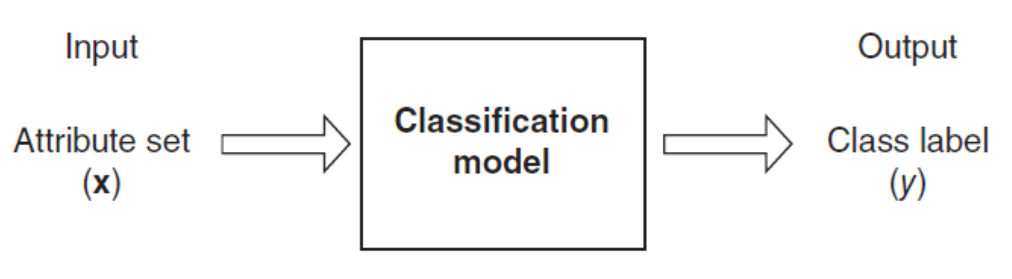
\includegraphics[scale = 0.6]{Images/classification.png}
    \caption{A schematic illustration of a classification task by Tan et al. \cite[p.~134]{DBLP:books/aw/TanSKK2019}.}
    \label{fig:classifiation}
\end{figure}


%\TODO{maybe difference opinion, sentiment, subjectivity?}
%According to Pang and Lee sentiment analysis "deals with the computational treatment of [...] opinion, sentiment, and subjectivity in text" \cite[p.~5]{DBLP:journals/ftir/PangL07}.  Pang and Lee suggest several applications for sentiment analysis, such as review-related websites, in addition to existing technologies such as recommendation systems, as well as business and government intelligence \cite[p.~8]{DBLP:journals/ftir/PangL07}.

\section{Sentiment Analysis}


\subsection{Definition}


Liu defines sentiment analysis, also known as opinion mining, as "the field of study that analyzes people's opinions, sentiments, appraisals, attitudes, and emotions toward entities and their attributes expressed in written text" \cite[p.~1]{liu_2015}. He states that entities include "products, services, organizations, individuals, events, issues, or topics" \cite[p.~1]{liu_2015}. He further analyzes the difference between sentiment and opinion, citing the Merriam-Webster dictionary. There, "sentiment is defined as an attitude, thought, or judgment prompted by feeling, while opinion is defined as a view, judgment, or appraisal formed in the mind" \cite[p.~2]{liu_2015}. Considering this definition, a subtle difference can be seen, where sentiment tends to be viewed more as a feeling, while an opinion is a more concrete view. Although this difference exists, sentiment analysis and opinion mining are still used interchangeably to refer to the same field. Liu defines the term opinion as an encompassing term that includes not only sentiment, but also additional information, such as the opinion holder. A more formal definition of an opinion by Liu can be seen in Equation \eqref{eq:opinion}.
\begin{equation}
    opinion = (e, a, s, h, t),
    \label{eq:opinion}
\end{equation}
where $e$ denotes an entity, $a$ is the target aspect of $e$, $s$ represents the sentiment, $h$ describes the opinion holder, and $t$ the time when the opinion was published \cite{liu_2015}. To further illustrate the difference, the example sentence "I like the display of my Dell laptop", published on 07.05.2022 by Max Mustermann is considered. Here, the entity $e$ is the target of the opinion, the Dell laptop, while $a$ is the specific attribute of the laptop that the sentiment relates to, the display. The sentiment $s$ is qualified as positive, the opinion holder $h$ is Max Mustermann, and the time $t$ is 07.05.2022, resulting in the quintuple (Dell laptop, Display, Positive, Max Mustermann, 07.05.2022). If an opinion does not target a specific aspect, but rather the entire entity, the aspect is defined as "GENERAL" \cite{liu_2015}. 


Liu identifies three different levels of analysis. The document level classifies an entire document as positive or negative, while assuming that it relates to a single entity, such as a product review. The next level is the sentence level, which determines the sentiment of each sentence, including neutral if it does not contain an opinion. The aspect level includes the entity and aspect with which an opinion is concerned \cite{liu_2015}.

Most research differentiates between two tasks in sentiment analysis. Pang and Lee, for example, differentiate between detection of polarity and detection of subjectivity. The most common form of polarity detection is called sentiment polarity classification, which aims to label an opinionated document as either positive or negative. Polarity may also be viewed as a multiclass problem, where the degrees of positivity are considered, as well as the neutral class, which Pang and Lee describe as the middle ground between positive and negative. Subjectivity detection, on the other hand, seeks to determine whether a given text contains a subjective opinion or is objective. Pang and Lee note that they make a distinction between neutral and objective, the latter being a lack of opinion \cite{DBLP:journals/ftir/PangL07}. Other researchers such as Liu define neutral as being the lack of opinion, noting that an objective sentence may still imply sentiment \cite{liu_2015}. Especially in human-coded data sets, the difference between objective and neutral is often problematic. For example, Nakov et al. instructed their coders to determine whether a sentence is objective, positive, negative, or neutral. Once Nakov et al. used this data set in their sentence polarity task, they combined sentences with an objective and neutral score to one class, as the coders often confused the two classes \cite{nakov-etal-2013-semeval}.

\begin{figure}
    \centering
    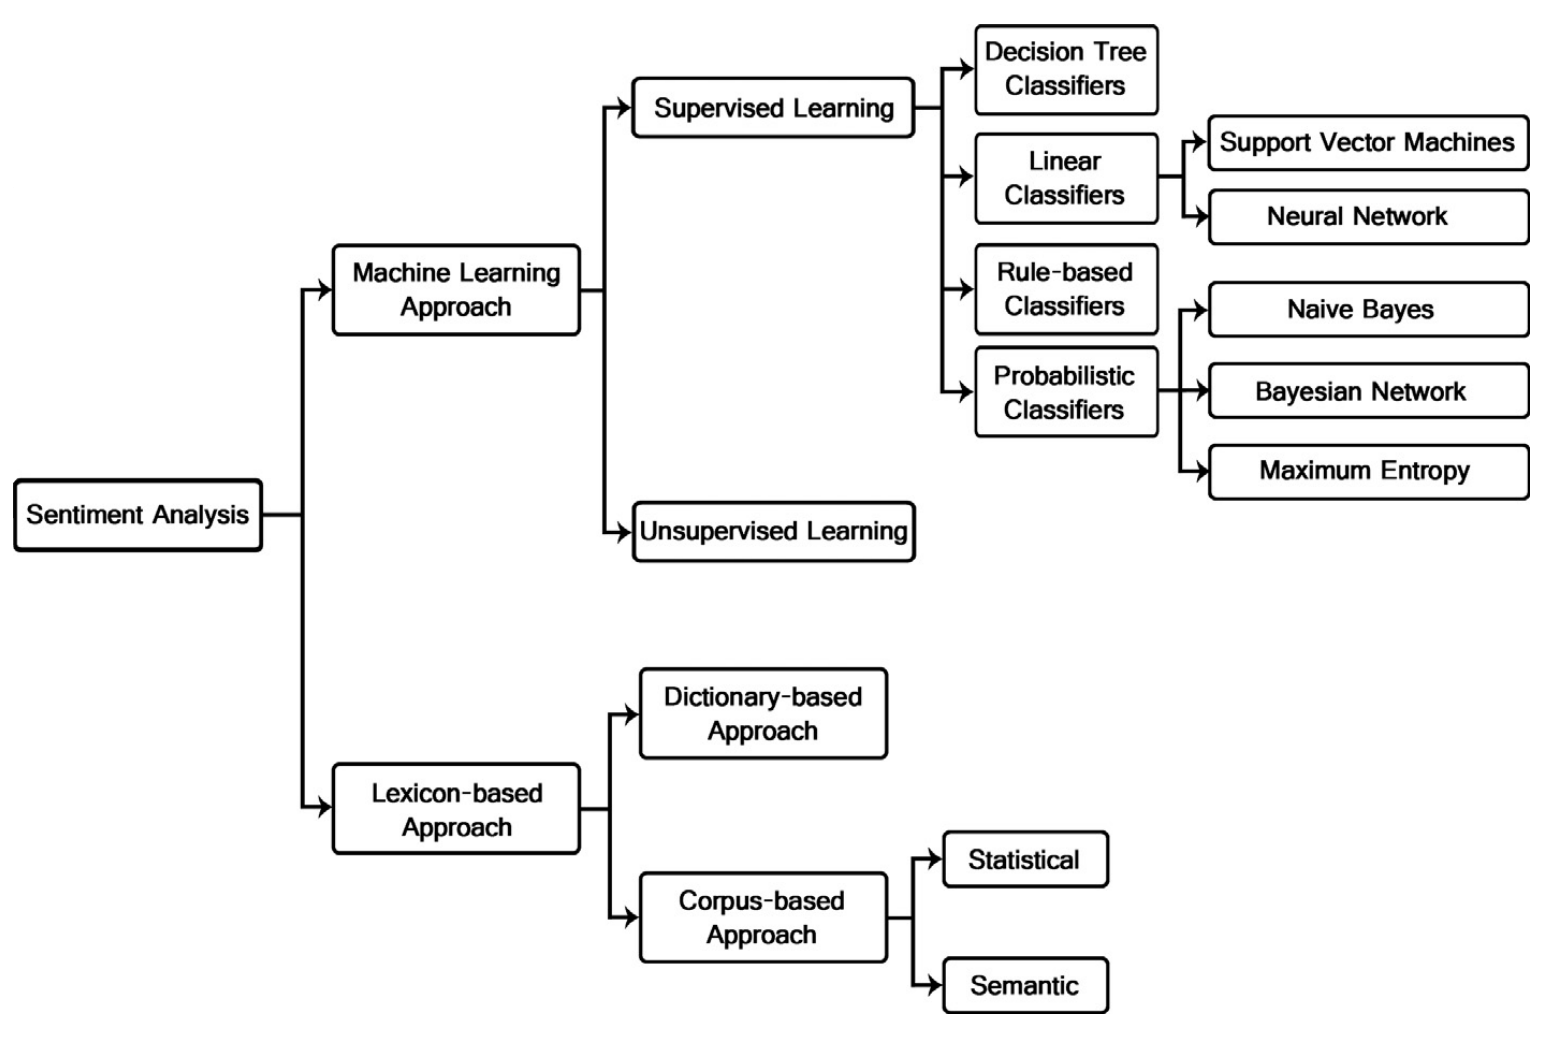
\includegraphics[scale=0.3]{Images/classification_techniques.png}
    \caption{Sentiment classification techniques by Medhat et al. \cite{MEDHAT20141093}.}
    \label{fig:classifiers}
\end{figure}

\subsection{Approaches}
For polarity classification, Medhat et al. divide techniques into three categories, machine learning, lexicon-based, and hybrid \cite{MEDHAT20141093}. Giachanou and Crestani identify a fourth technique, graph-based methods, \cite{DBLP:journals/csur/GiachanouC16}, which are not considered in this thesis. The most important classifiers are shown in Figure \ref{fig:classifiers}. 

\subsubsection{Machine learning classifiers}
\label{sub:fund_mach}
In general, the machine learning approach treats sentiment analysis as a text classification problem, employing training data to classify unknown instances. Supervised machine learning utilizes labeled training documents together with classifiers such as Naive Bayes. Because it can be difficult to generate a large number of labeled training data, unsupervised approaches are also applied, which rely solely on unlabeled data \cite{MEDHAT20141093}. The supervised methods are further subdivided. According to Tan et al., probabilistic classifiers, such as Naive Bayes and Logistic Regression, "make use of probability theory to represent the relationship between attributes and class labels" \cite[p.~414]{DBLP:books/aw/TanSKK2019}. Linear classifiers, on the other hand, try to find a hyperplane to separate instances from different classes \cite{MEDHAT20141093}. Decision Tree Classifiers, such as Random Forest, use attribute values to divide data into a tree structure. Finally, rule-based classifiers utilize a set of rules to classify an instance \cite{DBLP:books/aw/TanSKK2019}.

Feature selection is one of the essential parts of machine learning, as a classifier relies on the provided attributes. Giachanou and Crestani identify several different possible features for Twitter sentiment analysis: (1) Semantic features, for example, sentiment words and negations, which are extracted using lexicons; (2) Syntactic features, such as the presence of a word or term; (3) Stylistic features, which include emoticons and punctuation; and (4) Twitter-specific features, for example, hashtags or the number of replies \cite{DBLP:journals/csur/GiachanouC16}. For syntactic features, approaches differentiate on how to implement them. Some approaches look at each word of a tweet separately, which is called the unigram model, while others combine two (bigram model) or more words (n-gram model) as a combined feature.

\subsubsection{Lexicon-based methods}
\label{sub:fund_lex}
As stated previously, the lexicon-based approach needs a sentiment lexicon to identify sentiment words and their polarities. In addition, modifiers such as intensifiers and negations can be included to adjust sentiment values \cite{liu_2015}. There are three different methods for building a sentiment lexicon, which are outlined by Medhat et al. There is the manual collection of words, which is very time-intensive. A dictionary-based approach, which starts with a small list of sentiment words, can also be used. It subsequently searches dictionaries for synonyms and antonyms of the sentiment words, maintaining the orientations for synonyms and reversing them for antonyms. The found words are then added to the list and considered in the next iteration. The corpus-based approach utilizes context-specific orientations along with a list of opinion words to find other opinion words in a large corpus. It is based on sentiment consistency, which assumes that adjectives conjoined by "and" have the same polarity, while "but" would signify opposing polarities. This approach can be further subdivided into statistical approaches, which find words using statistics, and semantic approaches, which utilize semantic relationships \cite{MEDHAT20141093}.

\subsubsection{Hybrid methods}

Hybrid methods combine lexicon-based and machine learning methods to balance their disadvantages. Lexicon-based methods are inherently static, as they depend on a set list of words. If a tweet contains words that do not appear in the lexicon, the lexicon-based method can not classify it. On the other hand, a machine-learning method requires a large amount of labeled training data that is not easy to obtain manually. Approaches include using the lexicon-based score as an additional feature for the machine learning classifier, or employing multiple different classifiers by, for example, voting on the result \cite{DBLP:journals/csur/GiachanouC16}.


\section{Twitter}
Twitter is a microblogging service, which allows users to send messages, so-called "tweets", containing text, media, and URLs \cite{DBLP:journals/csur/GiachanouC16}. It is one of the largest social media platforms with 330 million monthly users in the first quarter of 2019, who posted 500 million messages daily \cite{twitter:users}. According to Pew Research Center, 23\% of U.S adults used Twitter, and the platform also had the second lowest age gap among the most popular social media platforms \cite{pew:socialmedia}. The length of a tweet was originally restricted to 140 characters until the company expanded the size to 280 characters in 2017 \cite{twitter:characters}. Due to this, Twitter offers a large number of short messages on varying topics made by varying user groups. 

Figure \ref{fig:example_tweet} shows an example of a tweet made by NASA for the Phoenix mission. An account is identified by its unique username, in the example tweet "@MarsPhoenix". There are several ways to interact with a tweet. A tweet can be (1) replied to, (2) retweeted, which shares the tweet to a user's profile, (3) quoted, which adds a comment to the retweet, or (4) liked. Other users can also be mentioned in a tweet, with their username being identified by the "@" character. 

\begin{figure}
    \centering
    
\includegraphics[scale=0.3]{Images/twitter_image.png}
    \caption{Picture of a tweet made by the @MarsPhoenix account \cite{twitter:tweet}.}
    \label{fig:example_tweet}
\end{figure}

Twitter's characteristics lead to challenges when applied to sentiment analysis, which are outlined by Giachanou and Crestani. The short length of tweets differs from other domains often used in sentiment analysis, such as movie reviews, which are much longer. Bermingham and Smeaton concluded that classification of sentiment on microblogs is easier than classifying longer documents \cite{microblogs}.

The informal nature of Twitter and its length restrictions frequently lead to abbreviations, slang, and misspellings, which must be considered. Especially emphatic lengthening, which refers to the usage of repeated letters in order to amplify a word, for example, "gooood", is very common in Twitter \cite{DBLP:journals/csur/GiachanouC16}. These characteristics lead to data sparsity, since many terms appear infrequently over an entire corpus of tweets \cite{DBLP:journals/csur/GiachanouC16}. Tan et al. define that for sparse data, most attribute values of a data object are 0 \cite{DBLP:books/aw/TanSKK2019}. Applied to sentiment analysis, the vast majority of observed words, and thus features, do not appear in a tweet. Saif et al. observed that 93\% of the words in their Twitter corpus occurred less than 10 times, compared to 78\% in movie review data \cite{data_sparsity}. 

Twitter offers two APIs to retrieve and analyze Twitter data, REST and streaming \cite{DBLP:journals/csur/GiachanouC16}. There currently are three different access levels, which provide different rates and limits. The elevated level, for example, allows the retrieval of up to 2 million tweets per month \cite{twitter:about}. The REST API provides a short-lived connection, through which several functionalities can be accessed, such as the lookup, creation, and deletion of tweets. Most importantly, it can also be used to search for tweets. Twitter differentiates between recent search, which provides access to public tweets posted in the last week, and full-archive search, which enables access to every tweet ever made. For full-archive search, academic research access is needed. Tweets can be filtered according to parameters such as language, content, and type (e.g. retweet) \cite{twitter:search}. 

On the other hand, the streaming API allows developers to access a real-time stream of tweets, which can be filtered using rules \cite{twitter:stream}. All information is returned in a JSON format, which can be easily parsed by many programming languages. Thus, the Twitter API provides a great method to collect large amounts of tweets \cite{DBLP:journals/csur/GiachanouC16}.





\iffalse 
\chapter{Methodology}
\label{cha:Chapter4_Methodology}


Length: 20-25 pages

Effort: 8 weeks+

Teilung zwischen Methodik (eher abstrakt) und Implementierung
Damit beginnen --> also mit Implementierung

Questions:
\begin{itemize}
\item Structure --> differentiation between getting the data, analysing the data and evaluating the results ok? --> Kann man machen
\item General idea: ``Readers should be able to carry out the same procedure using the thesis'' --> level of detail, e.g. cloud services? --> Implementierung auch auf Github zur Verfuegung stellen, API auf hoeherem Level (was machen die Funktionen verwenden),
Falls Cloud: nur virtueller Rechner --> eher nicht wichtig, falls spezifische Dienstleistung z.B. OpenAI (KI, Parsing) --> dann detaillierter, eher Richtung Implementation
\item Case study --> Evaluation of accuracy based on one real life topic? Topic, e.g. Covid-19 pandemic, german elections (aufpasssen, Politik schwer!), ...? --> je nach Umfang auch mehrere (sollen sich unterscheiden, Covid sehr viele Bereiche), Tweets auch auf Englisch
\end{itemize}

Content
\begin{itemize}
\item Data 
\begin{itemize}
    \item What data does twitter provide, auch z.B. Likes, Retweets
    \item Data extraction, Cloud Services --> spezifischer Dienst?
\end{itemize}
\item Analysis
\begin{itemize}
    \item Lexicon-Based Method
    \item Machine Learning Based Method
    \item Hybrid Method
\end{itemize}
\item Evaluation
\begin{itemize}
    \item Parameters --> objektive Kriterien, Qualitaet der Analyse Methode + Begruendung der Kriterien, Komplexitaet (Laufzeitkomplexitaet ja, Implementierung --> an sich nicht schlimm, aber robust? Abstuerze?)
    \item Case Study
    \item Qualitaet der Ergebnisse --> gut/schlecht, kann das akkurat erkannt werden?, evtl. menschliche Analyse, schoener: auf subjektive Einschaetzung verzichten
    \item Comparison with human tweets labeled by humans?
\end{itemize}
\end{itemize}


Analysis
\begin{itemize}
    \item Lexicon-Based Method
    \begin{itemize}
    \item General approach: Multiple lexicons with different topics, positive/neutral/negative
    \begin{itemize}
        \item Sentiment Words --> List of words with polarity, e.g. good
        \item Negation Words --> Words that negate the polarity of other words, e.g. not
        \item Intensity words --> Words that amplify the polarity, e.g. very
        \item Emoticons
    \end{itemize}
    \item Find the above word types in tweet
    \item Adjust polarity of sentiment words based on negation and/or intensity
    \item Calculate average of polarities including emoticons
    \item Example: The weather today is very terrible but the sound of rain is delightful.
    \begin{itemize}
        \item Sentiment of "very terrible": amplified negative (e.g. -2)
        \item Sentiment of "delightful": positive (e.g. +1)
        \item Overall: -2 + 1 = -1 --> negative
    \end{itemize}
    \item Comparison of different sentiment lexicons?
    \item Stop words --> needs, wants, etc. --> automatically negative (except for negation?)
    \item common idioms?
    \item slang
    \end{itemize}
    \item Machine Learning Based Method
    \begin{itemize}
        \item Naive Bayes --> probabilistic, multiple classes
        \begin{itemize}
            \item Based on Bayes theorem with conditional independence, add-one (laplace) smoothing, calculate P(x|y)
            \item Look at every word contained in tweet, apply formula to known words:
\[P(\mathrm{w}_{i}^{}|c) = \frac{count(\mathrm{w}_{i}^{}, c)+1}{(\sum_{w\in V}^{} (count(w,c)) + \left| V \right|} \]
            \item w = word, c is class (negative, positive), V is vocabulary of all known words
            \item Train with labelled tweets
           \[ \mathrm{c}_{NB}^{} = argmax_{c \in C}  P(c) \prod_{i \in positions}^{} P(\mathrm{w}_{i}^{}|c)\]
          
           
        \end{itemize}
        \item Logistic Regression? --> discriminative, binary classes
        \begin{itemize}
        \item Advantage: Not as many assumptions --> works better even when some features are correlated
        \end{itemize} 
        
    \end{itemize}
    \item Hybrid Method
    \begin{itemize}
        \item Approach 1 --> use lexicon-based score as an additional feature for the classifier (even if 0, it still can be classified)
        \item Combine the previous two or e.g. use a different classifier if that works better?
    \end{itemize}
\end{itemize}
\

New Learnings
\begin{itemize}
    \item Evaluation of different classifiers --> (J48), Naive Bayes (gaussian + multinominal distribution), Support Vector Machine, Logistic Regression, Random Forest
    \item Currently best: Naive Bayes with a multinomial distribution, 78.67\% of 4726 instances correct
    \item Caveats: Training for SVM and Logistic Regression not possible with all 1.2MM tweets --> system memory/runtime
    \item TODO: currently the ML method only recognized positive and neutral, more test instances?
    \item Lexicon Method: 75.68\% accurate on 9057 instances (includes neutral)
\end{itemize}

RandomForest
\begin{itemize}
    \item Collection of tree-structured classifiers
    \item Each tree depends on values of a random, independent vector
    \item Output is class selected by most trees
\end{itemize}

Questions
\begin{itemize}
    \item Fundamentals vs. Methodology: Wo z.B. Classifiers erklären?
    \item Welche Classifier wie vertiefen?
    \begin{itemize}
    \item Tabelle die Classifier vergleicht
    \item Kurze Erklärung aller Classifier?
    \item "Besten" Classifier tiefer erklären?
    \item z.B. Naive Bayes: Multinominale und Gaußsche Verteilung vergleichen/erklären?
    \end{itemize}
    \item Spezifische Bibliothek erwähnen (weka), Filter genauer (speichert nur 15000 Wörter, die mindestens 10x vorkommen, lowercase)?
    \item Daten beschreiben: Referenz + kurzer Überblick (Anzahl positiv/neutral/negativ, Themen, Zeitraum, bei Testdaten die Methode zur Klassifikation)
\end{itemize}
\fi




    

        
    
        
        













\chapter{Methodology}
\label{cha:Chapter4_Methodology}
The primary objective of this thesis is the implementation and evaluation of three different methods for sentiment analysis, more specifically, the task of sentiment polarity classification. The focus lies on binary classification, as this is the most commonly used implementation, especially for machine learning methods. Additionally, only the document/sentence level is considered. Due to Twitter's length restriction, the difference between the document and sentence level is diminished, as a tweet will often consist of only one sentence. Additionally, a tweet often concerns only a single entity, which can be identified by the presence of a word or hashtag \cite{DBLP:journals/csur/GiachanouC16}. To summarize, this thesis focuses on sentiment polarity classification on the document/sentence level.

\section{Lexicon-Based Method}
As mentioned in section \ref{sub:fund_lex}, lexicon-based methods rely on an algorithm to predict the sentiment of a tweet using one or multiple lexicons. One motivation for this approach outlined by Taboada et al. is domain independence. If a machine-learning classifier is trained using data from one single source, or one single type of source, it may affect which words the classifier deems as most significant. Taboada et al. analyzed the most important positive and negative features from a Support Vector Machine classifier trained on movie reviews. Among the most negative features were "2", "video", "tv" and "series". In a movie context, these features make sense, as sequel movies, as well as movies adapted from a video game or television series, are generally less liked. But if the classifier is to be domain-independent, these specific features are irrelevant or even misleading \cite{taboada}. Finn and Kushmerick looked at domain transfer by classifying documents assigned to a different topic from the one the machine learning classifier was trained on. While they achieved high accuracy for single-topic classification, the domain transfer resulted in much lower accuracy \cite{Finn03learningto}.

Another motivation is the ability to take context and sentence structure into account. For example, modifiers, such as negations and intensifiers, change the sentiment of the connected word and should be considered. In machine learning, bigrams can be applied to combine two words into a single feature, such as "not good", to learn the effect of certain combinations such as negations. While this is an improvement, negations often are not located directly next to the sentiment word they affect, and the training data would need to contain a sizeable amount of different combinations to be able to use it as significant features \cite{taboada}.

In this thesis, the lexicon-based method uses four different word classes to calculate sentiment. The approach is based on sentiment words and their modifiers, in this approach, negations and intensifiers. Additionally, emojis are considered, as there is a high usage of emojis on Twitter. Because Twitter is an informal type of medium, words are preprocessed to prevent cases such as misspelling and emphatic lengthening from affecting the detection of sentiment words.

\subsection{Word Classes}
This chapter shortly explains each word class employed and gives examples in order to showcase their use.

\subsubsection{Sentiment Words}
Sentiment words, also called opinion words, carry a positive or negative semantic orientation. Polarity-based lexicons only express whether a word is positive or negative, while a valence-based lexicon also determines the strength of a word. For example, a polarity-based lexicon would not differentiate between "bad" and "terrible", as both are negative, while a valence-based lexicon would establish "terrible" as having a stronger negative sentiment \cite{DBLP:conf/icwsm/HuttoG14}.

\subsubsection{Intensifiers}
Taboada et al., according to Quirk et al., name two types of intensifiers, amplifiers and downtoners. While amplifiers such as "very" increase the related sentiment, downtoners such as "barely" diminish it. Intensifiers should take the related sentiment into account and scale it accordingly \cite{taboada}.

\subsubsection{Negations}
Negations reverse the polarity of the corresponding sentiment, for example, turning the positive sentiment "good" into the negative sentiment "not good". It is important though to note that negations do not necessarily appear right in front of the sentiment word they reverse, for example, an intensifier can be in between as in "not very good" \cite{taboada}.

\subsubsection{Emojis}
The Cambridge Dictionary defines an emoji as "a digital image that is added to a message in electronic communication in order to express a particular idea or feeling" \cite{cambridgeEmoji}. As Hu et al. found out, "the most popular intentions are expressing sentiment, strengthening expression, and adjusting tone" \cite[p.~109]{Hu_Guo_Sun_Nguyen_Luo_2017}. The use of emojis on Twitter has been steadily increasing, with 21.54\% of global tweets containing at least one emoji in the month of December 2021 \cite{emojiStatistic}. Thus, it is clear that emojis are an important part of a tweet's overall sentiment and need to be taken into consideration.








\section{Machine Learning based Method}
\TODO{kind of similiar to related work?}
Machine Learning is a popular approach in Sentiment Analysis. Pang et al. were one of the first to employ and compare the use of different machine learning classifiers. Their classifiers worked in the movie review domain, where they were able to achieve high accuracy \cite{pang-etal-2002-thumbs}. Go et al. proved that machine learning classifiers also achieved high accuracy in the Twitter domain, which is why a machine-learning based approach has to be considered.

\iffalse
\begin{figure}
    \centering
    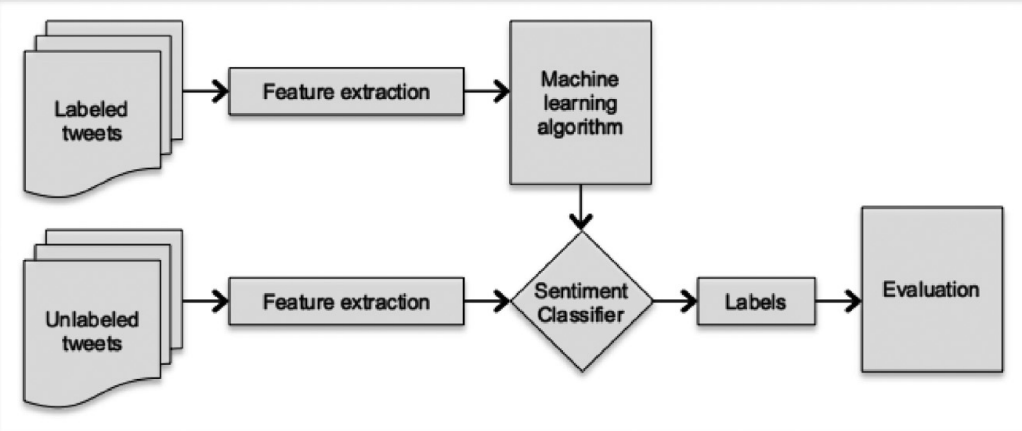
\includegraphics[scale=0.5]{Images/ML_approach.png}
    \caption{Caption}
    \label{fig:ml_approach}
\end{figure}

\fi

\begin{figure}
    \centering
    \tikzset{
  every shadow/.style={
    fill=none,
    shadow xshift=0pt,
    shadow yshift=0pt}
}
\tikzset{module/.append style={top color=\col,bottom color=\col}}

\smartdiagramset{uniform color list=white for 6 items,
    back arrow disabled=true, module minimum width=2cm,
    module minimum height=2cm,
    module x sep=3cm,
    text width=2cm,
    uniform arrow color=true,
    arrow color=black,
    additions={
        additional item shape=rectangle,
        additional item offset=0.5cm,
        additional item width=3cm,
        additional item height=2cm,
        additional item text width=3cm,
        additional item fill color=white!20,
        additional item border color=black,
        additional arrow color=gray,
        additional arrow tip=stealth,
        additional arrow line width=1pt
      }
    }
    \smartdiagramadd[flow diagram:horizontal]{Tokenization, Stop Word Filtering, URL/Hashtag Removal, Stemming, Vectorization, Classification}
    {below of module5/Word Frequency vs. Presence, below of module1/Unigrams vs. Bigrams} 
    \smartdiagramconnect{->}{module5/additional-module1}
    \smartdiagramconnect{->}{module1/additional-module2}

    \vspace{25mm}

   \caption{Process for machine-learning based method.}
    \label{fig:my_label}
\end{figure}


\subsection{Tokenization}
The machine-learning classifier relies on features, also called attributes, which have to be extracted from the training data. In Twitter, these features most often are syntactic features, such as words. Tokenization refers to the extraction process of words out of a tweet/sentence \cite{DBLP:journals/csur/GiachanouC16}.  Here, the models also differentiate between a feature consisting of only one word, also called unigram, or two (bigram) or more words (n-gram). In this thesis, both models are looked at, and words are tokenized based on whitespace.
\subsection{Stop Word Filtering}
Because every word is treated as an attribute, some words can be removed in advance to improve both data sparsity and the feature size. Words with low impact on the sentiment of a sentence, such as "the" and "is", are referred to as Stop words and can thus be ignored \cite{DBLP:journals/csur/GiachanouC16}. Although there are pre-compiled lists of Stop Words, these often are outdated and not Twitter specific. Additionally, Saif et al. observed that the usage of pre-compiled lists reduced the accuracy of classification performance and recommended a dynamic solution, which considers the number of times a word appears over the data set \cite{data_sparsity}. 

\subsection{URL/Hashtag Removal}
Tweets often contain URLs of the media, article, etc. the tweet is concerned with. Because these links in itself don't affect the sentiment, they are too ignored. Additionally, tweets often contain a hashtag, which indicates that the tweet is concerned with specific topic. The hashtag character "\#" is removed, to not differentiate between words such as \#good and good and thus further reduce data sparsity and feature size.
\subsection{Stemming}
Tweets as an informal message often contain misspelled or otherwise modified words \cite{DBLP:journals/csur/GiachanouC16}. By using word stemming, which, according to Lovins, "reduces all words with the same root (or, if prefixes are left
untouched, the same stem) to a common form" \cite[p.~22]{Lovins1968DevelopmentOA}, different cases or spellings of the same word can be reduced to one common feature, which, again, reduces data sparsity.

\subsection{Vectorization}
\TODO{source}
Vectorization is the process of converting tweets into a format that is readable for the classifier. This includes the definition of data types, its representation and more. Additionally, the assigned value of a tweet also differs between using the binary presence of a word, or its frequency in a tweet \cite{DBLP:journals/csur/GiachanouC16}. In this thesis, both approaches are considered.

\subsection{Classification}
Once the training data has been preprocessed and turned into features, the task of training the models can begin. The classifiers chosen are Naive Bayes using the Gaussian Distribution, Naive Bayes using the multinomial Distribution, Random Forest, Logistic Regression and Support Vector Machine. Because the classifiers may have different runtimes, each classifier is first evaluated using a small subset of training data, to obtain a first impression of the training runtime. After this, the data size is gradually increased, until the entire data set was used, or the process becomes too resource intensive. Once the appropiate training size is found, the parameters of each classifier are evaluated, to improve both performance and accuracy. If the performance can be improved, the training size is adjusted accordingly. Once the optimal parameters and training size are found, the classifiers are evaluated and compared. To facilitate a better comparison, the classifiers are evaluated both using their maximum training size, as well as the same minimum training size.

The following sections explain each machine-learning method in more detail.

    \subsubsection{Naive Bayes}
        Naive Bayes is a probabilistic, generative classification model, as it does not directly estimate the probability from the training data. It is based on the Bayes theorem, which is shown in Equation \eqref{eq:bayes}:
        \begin{equation}
            \label{eq:bayes}
            P(c_j|d_i) = \frac{P(c_j) * P(d_i|c_j)}{P(d_i)},
        \end{equation}
        where $c_j$ is a class label and $d_i$ is the document, in our case a tweet. \cite{DBLP:books/aw/TanSKK2019}. 
        
        Bayes theorem allows to calculate the posterior probability $P(c_j|d_i)$, which Tan et al. describe as "the probability of observing a class label $c_j$ for a data instance given its set of attribute values $d_i$" \cite[p.~418]{DBLP:books/aw/TanSKK2019}. 

        To calculate the posterior probability, the class conditional probability $P(d_i|c_j)$ is needed, which describes the probability of observing a set of attribute values given a class. Because of this indirect calculation, Naive Bayes is a generative model. One approach to calculate the class conditional probability outlined by Tan et al. is to ''consider the fraction of training instances of a given class for every possible combination of attribute values'' \cite[p.~419]{DBLP:books/aw/TanSKK2019}. With a large number of attributes and values, this method becomes computationally infeasible due to the exponential growth of combinations \cite{DBLP:books/aw/TanSKK2019}.

        Due to this, the Naive Bayes assumption is employed to estimate the class conditional probability. Naive Bayes uses conditional independence, which states that attribute values are only dependent on the class label and not each other. Thus, the class conditional probability can be calculated by using Equation \eqref{eq:naive_assumption}:
        \begin{equation}
            \label{eq:naive_assumption}
            P(d_i|c_j) = \prod_{t=1}^{n}P(w_{t}|c_j),
        \end{equation}
        with $d_i$ containing $n$ attributes $\{w_1,w_2,...,w_t\}$ \cite{DBLP:books/aw/TanSKK2019}.

        Furthermore, $P(d)$ remains constant for every class label $c$, so the class that maximizes Equation \eqref{eq:naive_final} is chosen: 
        \begin{equation}
            \label{eq:naive_final}
            P(c_j|d_i)\propto P(c_j)\prod_{t=1}^{n}P(w_{t}|c_j) 
        \end{equation}   
        
        $P(c_j)$ denotes the prior probability and thus the distribution of class labels, which can be obtained using prior knowledge or the training data.
        
        There are different models on how to implement the Naive Bayes assumption for text classification. In this thesis, the Gaussian Naive Bayes and Multinomial Naive Bayes are discussed. 
        
        The Gaussian Naive Bayes assumes that numeric attributes, such as word count, are distributed according to the normal distribution, also called Gaussian distribution \cite{nb_gauss}. According to Evans et al., "it was originally developed as an approximation to the binomial distribution when the number of trials is large and the Bernoulli probability p is not close to 0 or 1". \cite[p.~143]{evans2011statistical}. It is described by two parameters, the mean $\mu$ and the standard deviation $\sigma$ \cite{evans2011statistical}. Applied to Naive Bayes, it results in Equation \eqref{nb:gauss}:
        \begin{equation}
        \label{nb:gauss}
            P(w_t = v|c_j) = \frac{1}{\sqrt{2\pi}\sigma}e^{-\frac{(v.\mu)^2}{2\sigma^2}},
        \end{equation}
        with $v$ denoting the number of times $w_t$ appears in the to be classified document \cite{nb_gauss}.
        
        In order to calculate Equation \eqref{nb:gauss}, the mean $\mu$ and the standard deviation $\sigma$ have to be estimated for each numeric attribute given the class. The two parameters can be approximated by using the sample average and sample standard deviation of the training data. Once these two parameters are calculated for every attribute and class, unknown instances can be classified using Equation \eqref{nb:gauss} in conjunction with Equation \eqref{eq:naive_final} \cite{nb_gauss}.
        
        According to McCallum and Nigan, "the multinomial model captures word frequency information in documents" \cite[p.~3]{Mccallum1998}. By considering not only if a word is present but also how often it is present, the additional information may have an advantage. They describe the document as being "an ordered sequence of word events, drawn from the same vocabulary V" \cite[p.~3]{Mccallum1998}, with its length being independent of class. Using Naive Bayes, we assume that every word event is independent.
        
        According to Evans et al., "the multinomial variate is a multidimensional generalization of the binomial. Consider a trial that can result in only one of $k$ possible distinct outcomes, labeled $A_i, i = 1,...,k$. The outcome $A_i$ occurs with probability $p_i$. The multinomial distribution relates to a set of n-independent trials of this type." \cite[p.~135]{evans2011statistical}.
        
        Applying this to the model, McCallum and Nigan state that "each document $d_i$ is drawn from a multinomial distribution of words with as many independent trials as the length of $d_i$" \cite[p.~3]{Mccallum1998}. Using the multinomial distribution, the class conditional probability can then be calculated using Equation \eqref{eq:multinomial_bayes}:
        \begin{equation}
            \label{eq:multinomial_bayes}
                P(d_i|c_j) = P(|d_i|)|d_i|!\prod_{t=1}^{|V|}\frac{P(w_t|c_j)^{N_{i_t}}}{N_{i_t}!},
        \end{equation}
        
        with the document $d_i$ containing $|V|$ words $w_t$, $N_{i_t}$ being the number of times $w_t$ appears in $d_i$ and $c_j$ describing a class \cite{Mccallum1998}. 
        
        To estimate $P(w_t|c_j)$, the probability of a word $w_t$ given a class $c_j$, training instances are used to count the number of times a word appears in a class in Equation \eqref{eq:prob_word}:
        \begin{equation}
            \label{eq:prob_word}
                P(w_t|c_j) = \frac{1 + \sum_{i=1}^{|D|}N_{it} P(c_j|d_i)}{|V| + \sum_{s=1}^{|V|} \sum_{i=1}^{|D|}N_{is} P (c_j|d_i)} 
        \end{equation}
        with $D$ containing labeled training documents $(d_i,c_j)$, $N_{it}$ describing the number of times $w_t$ appears in document $d_i$, and $|V|$ containing all words \cite{Mccallum1998}.
        Equation \eqref{eq:prob_word} contains the posterior probability $P(c_j|d_i)$, which is the probability we want to calculate for unknown documents. Because we use labeled training documents, we know the class label, thus resulting in the posterior probability shown in Equation \eqref{eq:post_prob}:
        \begin{equation}
                \label{eq:post_prob}
                P(c_j|d_i)= 
                \begin{dcases}
                1,& \text{if } d_i \text{ was assigned the class label } c_j \\
                0,              & \text{otherwise}
        \end{dcases}
        \end{equation}
        Because of Equation \eqref{eq:post_prob}, Equation \eqref{eq:prob_word} only sums up the number of occurrences of a word in instances of a single class, as the occurrences in other classes are multiplied with 0. Thus, it can be simplified into Equation \eqref{eq:prob_word_simpler}:
                \begin{equation}
            \label{eq:prob_word_simpler}
                P(w_t|c_j) = \frac{1 + count(w_t, c_j)}{|V| + \sum_{s=1}^{|V|}count(w_s|c_j)} 
        \end{equation}

        with $count(w_t|c_j)$ counting the number of times a word $w_t$ appears in all training instances of a class $c_j$.
        
        By using Equation \eqref{eq:prob_word}, we calculate the word probability $P(w_t|c_j$). We utilize this in Equation \eqref{eq:multinomial_bayes} to calculate the class conditional probability $P(d_i|c_j)$ using the multinomial distribution. Finally, this allows us to estimate the posterior probability $P(c|d)$, as shown in Equation \eqref{eq:naive_final}. By selecting the class with the higher posterior probability, the classifier is able to make a prediction.
        
\subsubsection{Random Forest}
        According to Tan et al., Random Forest is an ensemble method that utilizes multiple base classifiers to take a vote on their predictions. The final prediction is then made by either averaging the vote or taking the majority vote. Random Forest applies a set of decorrelated decision trees by implementing two key characteristics \cite{DBLP:books/aw/TanSKK2019}.
        
        The first characteristic is bagging. Each tree is trained by a data set that was sampled from the original training data. Because the sampling is done with replacement and the samples must have the same size as the original training data, the sample will, on average, only contain 63\% of the original data \cite{DBLP:books/aw/TanSKK2019}.
        
        The selection of input attributes is the second characteristic. When a tree is being constructed, an attribute must be selected for splitting at each internal node. Random Forest randomly chooses a subset of attributes, from which the attribute with the maximum reduction in an impurity measure is chosen \cite{DBLP:books/aw/TanSKK2019}.
        
        Through these characteristics, Random Forest reduces the correlation of trees and thus the variance, because the trees use different data sets and input attributes \cite{DBLP:books/aw/TanSKK2019}. In Figure \ref{fig:tree}, a part of a tree generated by a Random Forest classifier can be seen. Here, the existence of a word is used as the attribute for splitting. If, for example, $hurts \geq 0.5$, the word $hurts$ exist in the document that is being analyzed, while $hurts < 0.5$ signifies that the word $hurts$ does not exist.
        
        \begin{figure}
        \centering
        \begin{tikzpicture}
        [
        grow                    = right,
    sibling distance        = 4em,
    level distance          = 9em,
    edge from parent/.style = {draw, -latex},
    every node/.style       = {font=\footnotesize},
    sloped
  ]
  \node [root] {}
    child { node [dummy] {}
      child { node [dummy] {}
        child { node [dummy] {}
            child { node [env] {$-1.0$}
                edge from parent node [below, align=center] {$studying < 0.5$} }
            child { node [env] {$+1.0$}
                edge from parent node [above] {$studying \geq 0.5$} }
            edge from parent node [below] {$will < 0.5$} }
        child { node [env] {$-1.0$}
                edge from parent node [above] {$will \geq 0.5$} }
        edge from parent node [below] {$hates < 0.5$} }
      child { node [env] {$-1.0$}
              edge from parent node [above, align=center]
                {$hates \geq 0.5$}}
              edge from parent node [above] {$hurts \geq 0.5$} };
\end{tikzpicture}
    \caption{Part of a tree generated by the Random Forest classifier.}
      \label{fig:tree}
\end{figure}
\subsubsection{Logistic Regression}
Logistic Regression calculates the posterior probability $P(c_j|d_i)$ directly, without relying on the class conditional probability like Naive Bayes, which is why it is a probabilistic discriminative model. In a binary model, the class label can be assigned by calculating the odds, as seen in Equation \eqref{eq:logistic_odds} \cite{DBLP:books/aw/TanSKK2019}:
        \begin{equation}
            \label{eq:logistic_odds}
                \frac{P(c=1|d)}{P(c=0|d)}.
        \end{equation}
If the odds are greater than 1, then the class label 1 can be assigned to document d, otherwise class 0 is assigned. Logistic Regression represents the odds using a linear predictor $z=w^Tx + b$, which results in equation \eqref{eq:logistic_linear}:
        \begin{equation}
            \label{eq:logistic_linear}
                \frac{P(c=1|d)}{P(c=0|d)} = e^z = e^{w^Td+b},
        \end{equation}
with the parameters $w$ and $b$ and $w^t$ signifying the vector transpose \cite{DBLP:books/aw/TanSKK2019}.

By substituting $P(c=0|d)$ with $1 - P(c=1|x)$ and solving for $P(c=1|d)$, we get Equation \eqref{eq:logistic_sigmoid}:
        {\begin{equation}
            \label{eq:logistic_sigmoid}
                P(c=1|d) = \frac{1}{1+e^{-z}} = \sigma(z).
        \end{equation}}
$\sigma(z)$ is called the sigmoid function, whose graph can be seen in Figure \ref{fig:sigmoid}.
        \begin{figure}
        \centering

\begin{tikzpicture}
\begin{axis}
[
    grid=major,   
    xmin=-10,
    xmax=10,
    axis x line=bottom,
    ytick={0,.2,.4,.5,.6,.8,1},
    ymax=1.2,
    ymin=-0.2,
    axis y line=middle,
    width=0.8\textwidth,
    height=0.6\textwidth,
    xlabel={$z$},
    ylabel={$\sigma(z)$}
]
    \addplot%
    [
        blue,%
        mark=none,
        samples=100,
        domain=-10:10,
        ultra thick
    ]
    (x,{1/(1+exp(-x))});
\end{axis}
\end{tikzpicture}
    \caption{Plot of sigmoid function $\sigma(z)$.}
      \label{fig:sigmoid}
\end{figure}
As seen in Figure \ref{fig:sigmoid}, $\sigma(z) \geq 0.5$ when $z \geq 0$, so if $z \geq 0$, we assign the instance $d_i$ to the class $c = 1$. The parameter $w$ defines the weight assigned to an attribute value, in this case the presence/frequency of a word. For example, if a word is irrelevant for a class, the classifier would assign a weight close to 0. The parameters are learned during training using the maximum likelihood estimation method. For each training instance $(d_i|c_i)$, the probability of observing the class label $c_j$ given the parameters $(w,b)$ is calculated. Assuming independence among training instances, these probabilities can be multiplied to a single equation, shown in Equation \eqref{eq:logistic_max}.
        \begin{equation}
            \label{eq:logistic_max}
                L(w,b) = \prod_{i=1}^{n}P(c_i|d_i,w,b).
        \end{equation}
        
Using the likelihood of all training instances $L(w,b)$, the parameters $(w*,b*)$ with the maximum likelihood are chosen, the sigmoid function and thus the posterior probabilities $P(c=1|d)$ and $P(c=0|d)$ can be estimated and the document classified \cite{DBLP:books/aw/TanSKK2019}.


\subsubsection{Support Vector Machine}
Tan et al. define the Support Vector Machine as a discriminative classifier. It is based on a separating hyperplane that, as the name suggests, tries to separate instances of two classes. Furthermore, it only uses a subset of the training instances, those nearest the borders and thus hardest to classify. These instances are called support vectors \cite{DBLP:books/aw/TanSKK2019}.

The hyperplane can be described by Equation \eqref{eq:hyperplane}:
    \begin{equation}
            \label{eq:hyperplane}
                w^Td + b = 0,
        \end{equation}
    where $d$ represents the attributes and $(w, b)$ are the parameters of the model \cite{DBLP:books/aw/TanSKK2019}. 
    
    There can be an indefinite number of hyperplanes, which is why it is necessary to choose one that has good generalization performance, which means that it can handle unseen instances. To do this, the margin of a hyperplane $B_i$ is calculated by drawing two hyperplanes, $B_i1$ and $B_i2$, parallel to $B_i$. The distance between the two hyperplanes is the margin of the hyperplane $B_i$, as seen in Figure \ref{fig:svm} \cite{DBLP:books/aw/TanSKK2019}. By choosing the hyperplane with the maximum margin, the classifier can allow for slight changes in data without immediately crossing onto the other side.

    \begin{figure}
        \centering
        \caption{Margin of a hyperplane in a two-dimensional data set by Tan et al. \cite{DBLP:books/aw/TanSKK2019}.
        \label{fig:svm}
        }
        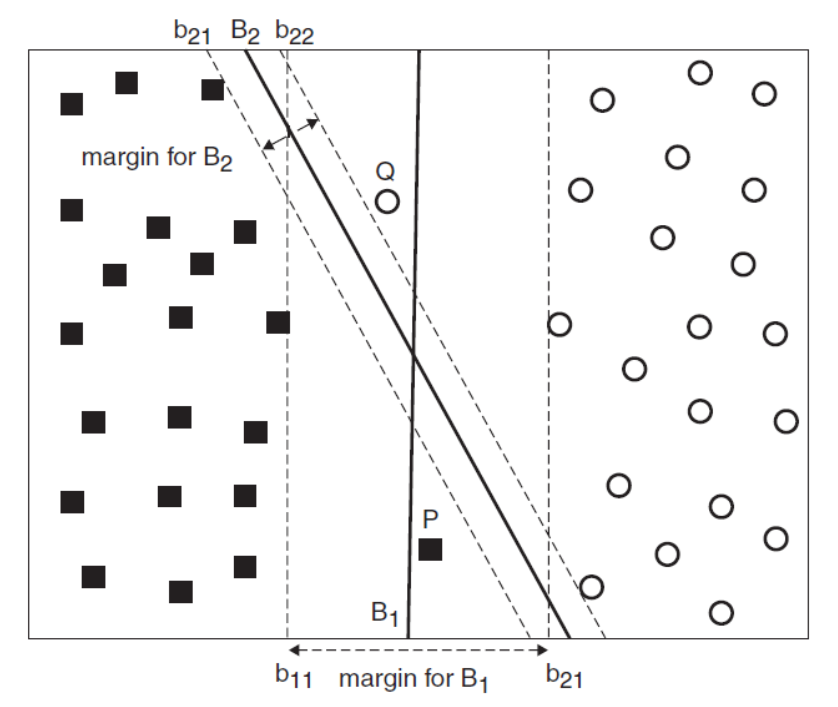
\includegraphics[scale=0.7]{Images/SVM_image.png}
    \end{figure}
    

    In Figure \ref{fig:svm}, the data can be separated by a linear hyperplane. This is not always the case, which is why a nonlinear Support Vector Machine transforms its input data $x$ into a new attribute space $\phi(x)$, in which a linear hyperplane can be constructed. Projected into the original attribute space, this hyperplane is a nonlinear decision boundary \cite{DBLP:books/aw/TanSKK2019}.
    
\section{Hybrid Method}
\TODO{Sources!}

\subsection{Approach 1}
The first approach consisted of using the score of a lexicon-based method as an additional feature of the machine learning method. If a tweet is to be classified, it is first scored using the lexicon-based method. The calculated score is then used as an additional feature for the machine learning method. This has the advantage of not relying solely on the static dictionaries used by the lexicon-based method, while still being able to take specific sentence structures like negation into account.
\subsection{Approach 2}
The second approach trains the machine learning classifier using tweets labeled by the lexicon-based method. The precision of a machine learning classifier is based on its training data, both its quality and its size \cite{DBLP:journals/csur/GiachanouC16}. Because machine learning classifiers perform better with more training data, using human-labeled training data is too expensive. Some approaches like Go et al. classify tweets as positive or negative based on the presence of certain emoticons and are thus able to train using 1.6 million tweets \cite{GoBHaHua2009}. By annotating tweets using a more accurate lexicon-based approach, the quality of the training data could increase and thus the machine learning classifier could become more accurate.
\subsection{Approach 3}



\chapter{Implementation}
\label{cha:Chapter5_Implementation}
\section{Test data}
The test data contained human-annotated tweets provided by two different sources and covered a wide variety of topics. In total, 10,372 tweets were used, of which 1,776 were labelled as negative, 4,968 as neutral, and 3,628 as positive.

\subsection{SentiStrength}
SentiStrength is a data set constructed in 2012 by Thelwall et al. to evaluate the second version of their SentiStrength algorithm, a lexicon-based classifier. As mentioned in section \ref{sub:related_lexicon}, they created data sets from multiple sources, including Twitter, BBC Forum, and other social media platforms. In this thesis, only the Twitter data set was used, which was labeled by one person \cite{10.1002/asi.21662}.

The data set contains three columns, an integer score of 1 to 5 for the positive score, a separate integer score of 1 to 5 for the negative score, and the tweet text \cite{10.1002/asi.21662}. Because a tweet can have both a considerable positive and negative score, an approach inspired by Saif et al. is used to convert it to a single polarity. A tweet is defined as positive if the positive score is at least 1.5 times higher than the negative one and vice versa. If neither score is at least 1.5 greater, the tweet is classified as neutral \cite{oro40660}. This resulted in 947 negative, 1,959 neutral, and 1,336 positive tweets.

\subsection{SemEval2013}
According to Giachanou and Crestani, "SemEval (Semantic Evaluation) is an ongoing series of evaluations of computational semantic analysis systems" \cite[p.~28:31]{DBLP:journals/csur/GiachanouC16}. In 2013, they constructed multiple data sets for both training and testing. They defined two subtasks, subtask A to determine the sentiment based on the context of a marked word/phrase, and subtask B to detect the sentiment based on the entire message. Because this thesis looks at tweets as a whole, only the second data set was utilized \cite{nakov-etal-2013-semeval}.

The tweets were parsed based on popular topics that were identified earlier from January 2012 to January 2013, and tweets that did not contain sentiment-bearing words were filtered out to lower class imbalance. The annotation of tweets was done by five Amazon Mechanical Turk workers, for subtask B the polarity selected by the majority was chosen \cite{nakov-etal-2013-semeval}. As the data set only provided the tweet IDs and not the text, the Twitter API was used to crawl the text for each tweet. This was not possible for every tweet contained in the data set, as some were already deleted or otherwise not available. This resulted in 6,130 tweets, of which 829 were negative, 3,009 neutral, and 2,292 positive.

\section{Lexicon-based Method}

\subsection{Lexicons}
In order to implement the word classes, four types of lexicons were used, which are described in the following sections.

\subsubsection{Sentiment lexicon}
The lexicon that contains sentiment words and their scores was chosen to be the valence-based dictionary VADER, constructed by Hutto and Gilbert. They created the lexicon by first gathering a list of common features in other lexicons, supplemented by additional aspects such as emoticons, acronyms, and slang. This list of 9000 features was then labeled by 10 independent human raters via Amazon Mechanical Turk on a scale of -4 to +4, with the average of all scores resulting in the final score. They removed all features whose score was zero and whose standard deviation was higher than 2.5, which resulted in a lexicon containing 7,500 features \cite{DBLP:conf/icwsm/HuttoG14}.

\subsubsection{Intensity lexicon}
For the intensifiers, the most common words from a list of English degree adverbs \cite{wiki:adverbs} were used and scored by a human rater. Amplifiers were given a rating above 1.0, while downtoners were given a rating between 0.0 and 1.0. For example, "almost" has a degree of 0.8, while "extremely" has a degree of 3.0.


\subsubsection{Negation lexicon}
For negations, a list was constructed that contained the most common negations. The list was based on a blog entry by the company Grammarly \cite{negations}. In addition to the words themselves, common spelling mistakes were included, such as a missing apostrophe for "isn't".

\subsubsection{Emoji Lexicon}
A lexicon constructed by Haak was used, which contains 198 emojis and their valence scores \cite{haak_dataset}. For example, the emoji "grinning face", which can be seen in Figure \ref{fig:emoji}, is assigned a positive score of +0.8. The score was calculated using the mean sentiment of tweets containing the emoji, which were classified using a lexicon-based method. Only emojis with more than ten occurrences and a standard deviation below 0.625 were considered. \cite{haak_article}.

\begin{figure}
    \centering
    
\includegraphics[scale=0.05]{Images/emoji_smile.png}
    \caption{Grinning face emoji by Twitter \cite{twitter:image}.}
    \label{fig:emoji}
\end{figure}



\subsection{Algorithm}

An algorithm was designed to classify tweets, which can be seen in Algorithm \ref{lexiconAlg}. Each tweet was first split using whitespace to separate each word. Then, each word was preprocessed. First, punctuation was removed, unless the word consisted of an emoticon/emoji. After each processing step, the word was searched for in the sentiment lexicon; if the word was not found, the process continued with the next step. Characters that appeared more than two times in a row were reduced to two times, in order to prevent emphatic lengthening. Additionally, characters were removed from the end of a word to prevent different word endings from affecting the algorithm, up to a minimum word length of 3.

Taking into account the four different word classes, the most important parts of a tweet that affect its sentiment were covered. There is one special case that had to be considered. The used lexicons define "no" as both a sentiment word and a negation, which is why the algorithm checked whether a sentiment word appeared after "no". If that was the case, the word "no" was skipped, as it was interpreted as a negation.

The total score of a tweet was calculated by adding the score of each sentiment word. The two words in front of a sentiment word were evaluated to determine if there was an intensifier and/or a negation. If so, the polarity and strength were adjusted accordingly. Additionally, if an emoji was detected, its sentiment was also added to the total score. The algorithm itself was implemented using Java.

Although this thesis focuses on polarity classification, the lexicon-based method was also able to return the strength of a given sentiment, as well as a neutral score of 0. A neutral score was only returned if no sentiment word could be detected or if the sum of detected sentiments was equal to 0.

\begin{algorithm}
  \caption{Lexicon-based algorithm used to return a positive, negative or neutral score for a given tweet.}\label{lexiconAlg}
    \begin{algorithmic}[1]
        \Function{analyze}{$tweet$}\Comment{Sentiment score of tweet}
            \State $SentimentLexicon \gets Dictionary[word][sentiment]$
            \State $NegationList \gets$ List of negation words
            \State $IntensityLexicon \gets Dictionary[word][intensity]$
            \State $EmojiLexicon \gets Dictionary[emoji][emojiSentiment]$ 
            \State $score \gets 0.0$
            \ForEach {$word \in tweet$}
                \State $word =$ preprocess($word$)
                \If{$word \in SentimentLexicon$} 
                 \If{$word ==$ "no"}
                        \ForEach {$nextWord \in$ next two words}
                        \If{$nextWord \in SentimentLexicon$}
                            \State Skip word
                        \EndIf
                        \EndFor
                \Else
                \State $polarity \gets 1$
                    \ForEach {$previousWord \in$ previous two words}
                        \If{$previousWord \in NegationList$}
                            \State $polarity = polarity * (-1)$
                        \Else
                            \If{$previousWord \in IntensityLexicon$}
                                \State $polarity = polarity * intensity$
                            \EndIf
                        \EndIf
                    \EndFor
                    \State $score = score + polarity * sentiment$
                \EndIf 
                \Else
                    \If{$word \in EmojiLexicon$}
                        \State $score = score + emojiSentiment$
                    \EndIf
                \EndIf 

            \EndFor
            \State \textbf{return} $score$
        \EndFunction
    \end{algorithmic}
\end{algorithm}


\section{Machine Learning based Method}

For the machine learning method, WEKA, developed at the University of Waikato in New Zealand, was chosen as the library. As described by Witten et al., "[t]he WEKA workbench is a collection of machine learning algorithms and data preprocessing tools [...]" \cite[p.~7]{weka}. It also includes tools for the entire process of data mining, such as preparation of data and evaluation. WEKA is implemented in Java, the version of the library used in this thesis was 3.9.6. Although it also offers a graphical interface only the Java library was used in this thesis \cite{weka}. Weka was chosen because of its large collection of both algorithms and tools for data mining, as well as ease of use through an extensive documentation.

Weka uses the Attribute-Relation File Format for its data, which contains a header describing the attributes, as well as the data itself, with one row containing one instance \cite{weka}. For this thesis, the class attribute was chosen to be nominal, either negative (-1.0) or positive (1.0), for a binary classification problem. Furthermore, the tweet text is added as a string attribute.

\subsection{Training data}
The training data for machine learning classifiers was created by Go et al. and consists of 1.6 million tweets \cite{GoBHaHua2009}. The tweets were parsed using the Twitter API by querying for positive or negative emoticons, such as ":)" and labeled as positive or negative depending on the emoticon. Furthermore, tweets containing both a negative and positive emoticon, as well as retweets were removed \cite{GoBHaHua2009}.

This resulted in 800,000 positive and 800,000 negative tweets that were periodically requested on no specific topic, thus covering a large number of topics \cite{GoBHaHua2009}.

\subsection{Tokenization}
For Tokenization, weka's NGramTokenizer was used, which splits a text into Ngrams of a certain size. The default delimiters, such as whitespace and "\textbackslash n", were used for splitting. The minimum size of the Ngram was set to 1 to include Unigrams, and the maximum size was set to 2 to include Bigrams \cite{weka}.
\subsection{Stop Word Filtering}
For Stop Word Filtering, both a list and a dynamic approach were used. A short list of common words such as "the" was manually collected and evaluated. To further reduce the word size, a limit was set for how often a word has to appear to be included, as well as a (soft) limit of total words. In the testing, a limit of 15,000 words was found to be optimal, with words appearing at least 20 times in the training data. This allowed for the greatest balance of performance and accuracy. This limit was set in weka's StringToWordVector, which is explained in more detail later.
\subsection{URL/Hashtag Removal}
??

\subsection{Stemming}
For stemming, weka's LovinsStemmer was used, which is based on the Lovins Stemmer \cite{weka}. This stemmer uses a two-step method, which first removes the ending, thus obtaining the stem. After this, similar stems are combined to account for different spellings. An example of this is "absorption", whose stem is "absorpt", while "absorbing" will result in "absorb"\cite{Lovins1968DevelopmentOA}.

\subsection{Vectorization}
In order to transform the text of a tweet into a suitable format for classifiers, weka's StringToWordVector filter is used. This filter transforms the string feature, the tweet's text, by parsing each word out of it using the previously defined NGramTokenizer. The words are then added to a dictionary, which stores all recognized words. In the data, the words are implemented as numeric attributes, with the value denoting the number of occurrences or its presence \cite{weka}.

For example, the tweet "i love it" would result in three attributes, the attribute "i", the attribute "love", and the attribute "it", as can be seen in Figure \ref{fig:arff_train}. The dictionary, and with it the attributes, are all determined by the training data. The test data set is also filtered, but only using the known words from the training data, no new words are added to the dictionary \cite{weka}.




\begin{figure}
    \centering
\begin{tikzpicture}
\vspace{5mm}
\node[draw, text width=6cm] at (0,0) { @relation TrainingData \\
                                        \medskip
                                        @attribute calculatedScore {-1.0, 1.0} \\
                                        @attribute tweetText string \\
                                        \medskip
                                        @data \\
                                        1.0,'i love it' \\
                                        -1.0,'i hate it' \\
                                        
                                        };
\node[draw, text width=6cm] at (8,0) { @relation TrainingData \\
                                        \medskip
                                        @attribute calculatedScore {-1.0, 1.0} \\
                                        @attribute i numeric \\
                                        @attribute love numeric \\
                                        @attribute it numeric \\
                                        @attribute hate numeric \\
                                        \medskip
                                        @data \\
                                        {0 1.0, 1 1 , 2 1 , 3 1} \\
                                        {0 0,   1 1 , 3 1 , 4 1}
                                        };
\end{tikzpicture}
\vspace{5mm}
    \caption{Example of training data in the ARFF format utilized by Weka before and after vectorization \cite{weka}.}
    \label{fig:arff_train}
\end{figure}

\subsection{Training}
For training, Weka's FilteredClassifier was used, which combines an arbitrary filter with an arbitrary classifier. The classifier classes used were "NaiveBayes" for Gaussian Naive Bayes, "NaiveBayesMultinomial", "Logistic" for Logistic Regression, "LibSV"M for Support Vector Machine and "RandomForest" \cite{weka}. For the Support Vector Machine, the LibSVM library had to be added to the project, as Weka only provided a wrapper class \cite{Chang2001}. Once a classifier was built, its file was saved. RandomForest resulted in large files, with the largest being 471 megabytes. For the evaluation, Weka's Evaluation class was used, which automatically calculated all needed measures \cite{weka}.
\section{Hybrid Method}

\subsection{Lexicon-based score as feature}
For the first approach, the best performing machine-learning classifier was used, which was multinomial Naive Bayes. The ARFF format was changed to include an additional numeric feature, the lexicon-based method's score. Because weka only allows values greater than or equal to zero for a numeric attribute, the maximum and minimum scores were \TODO{restricted} to -10 and +10, and each score was shifted by adding 10. Each training instance was evaluated using the lexicon-based method, and the score was added to the instance. For the test instances, the same procedure was applied.
\subsection{Label training data with lexicon-based method}
For the second approach, each training instance was scored using the lexicon-based method. Instead of adding an additional attribute though, the instance's class label was set to the lexicon-based method's score. Because we only considered two classes during classification, positive and negative, all instances with a neutral score were ignored. Furthermore, the score was normalized to -1.0 and 1.0, to fit the class labels. This resulted in 973,671 instances being used.




\chapter{Conclusion}
\label{cha:Chapter5_Conclusion}

\iffalse

Length: 1-2 pages

Effort: 1-2 days


Zusammenfassung der Ergebnisse, Ausblick --> was kann man noch machen, auf Ergebnisse aufbauen, weiterfuehrende Themen

Beim Erstellen der Arbeit --> nicht jeder Idee hinterherrennen, eher dann fuer Conclusion

Implementation source code --> muss nicht sein, kann auch ein link auf github sein

\fi

In this thesis, three different approaches for Twitter sentiment analysis were discussed, implemented, and evaluated based on a set of defined measures. The lexicon-based method utilized multiple lexicons for specific word classes and achieved an accuracy of 71.04\%. For the machine learning based method, several different classifiers and approaches were evaluated, with the Multinomial Naive Bayes, using word presence, unigrams, and bigrams, achieving the highest accuracy at 79.42\%. The hybrid methods combined the previous two approaches to balance their disadvantages, with the first approach using the lexicon-based score as an additional feature, and the second one labeling the training data with the lexicon-based method. The second method achieved the highest accuracy overall at 81.33\%, although both methods improved on the lexicon-based method and the machine learning based method.

\TODO{also depends on used lexicon, etc.}
The advantages and disadvantages were also discussed. The lexicon-based method was the least complex and resource-intensive method but also achieved the lowest accuracy. For use cases where performance is very important, such as analysis on large data sets, the accuracy is still high enough to be valuable, especially considering the domain-independence. If the goal is the highest accuracy possible, a machine learning-based classifier has to be involved. While the machine learning method requires more resources and is more complex, the accuracy is clearly superior. The hybrid methods were able to improve the accuracy slightly, although the additional complexity may often not be worth it.

\TODO{why did I not do these improvements, maybe}
There are a few improvements and new methods that can be explored. For the lexicon-based method, there are two types of possible improvements. First, the rate of non-detected tweets can be improved from the current circa 10\%. The inclusion of certain phrases or idioms such as "can't wait" are usually not covered by sentiment lexicons, but still appear often in tweets. Hashtags may also be utilized more effectively, as Twitter users often combine multiple words into a single hashtag, for example "\#itsNotCool". By not simply removing the hashtag, but also trying to extract words out of it, more tweets could be classified. Secondly, the correct classification of a detected sentiment can be improved, which accounts for circa 20\% of false classifications. Here, the focus should be on detecting negative sentiment, as this had a higher error rate. Capitalization could be used, as a sentiment word written fully capitalized can be amplified. Employing parts-of-speech tagging may also be important, as the sentiment of a word can change depending on its usage. For example, the word "break" has two different meanings depending on whether it is used as a verb or a noun ("to break something" compared to "to take a break"). Punctuation also affect sentiment, for example, a stronger score could be assigned for sentences with one or multiple exclamation marks.


\TODO{was ist der Unterschied zur normalen}
For the machine learning methods, deep learning could be a further improvement, due to its different representation of documents. Giachanou and Crestani compiled a list of deep learning approaches for Twitter Sentiment Analysis, which are capable of achieving high accuracy \cite{DBLP:journals/csur/GiachanouC16}. In addition, more Twitter-specific features could be used. Metrics such as the number of likes or comments may be able to indicate the sentiment of the corresponding text.

Hybrid methods can also be further developed. Classifier ensembles, which combine one or multiple machine learning classifiers and a lexicon-based classifier by, for example, voting on the final result, have been shown to improve performance compared to a single classifier \cite{DBLP:journals/csur/GiachanouC16}.

Research into Twitter sentiment analysis has been steadily growing the past few years and has proven to be a valuable source for sentiment analysis. Its combination of a wide variety of topics, short messages and large user base is very unique compared to traditional domains such as movie or product reviews. The interest in tracking sentiment and opinions on specific topics will only grow as social media platforms become larger and more influential, and thus research interest will continue to improve on the methods described in this thesis.

\TODO{licensing for data?}
\chapter{Code implementation}

The code implementation, as well as the data used, can be found in the GitHub repository under the URL: \url{https://github.com/hoffmatteo/thesis}.



% Literaturverzeichnis
\newcommand{\Literatur}{Bilbiography}
\addcontentsline{toc}{chapter}{\Literatur}
\nocite{*}
\bibliography{Literaturverzeichnis/literatur}


% Fügt Anhang zum Dokument hinzu
\appendix
\chapter{Implementation source code}
%\addcontentsline{toc}{chapter}{Appendix}
%\include{Appendix/Appendix}
%\include{Appendix/Code}


\end{document}
